% Lecture 7 notes: \input by notes.tex, \subimport'ed by the semester book.
% Exam questions (зачёт): 14–15 (порядок элемента: последовательное снижение, дерево
% произведений), 16 (поиск первообразного корня).
\begin{lecture}{7}{Порядок элемента и первообразные корни}

\section{Зачем нужны порядки и образующие}

В протоколе Диффи"--~Хеллмана (лекция~1) Алиса и Боб возводят в степень общедоступный элемент
$g \in \Znx{p}$. Стойкость протокола зависит не столько от $p$, сколько от \emph{порядка} $g$:
ключ $g^{ab}$ принимает не больше $\ord g$ различных значений, а во втором семестре мы увидим
(алгоритм Полига"--~Хеллмана), что дискретный логарифм вычисляется за время порядка
$\sqrt{q}$, где $q$ "--- наибольший простой делитель $\ord g$. Поэтому при выборе параметров
нужно уметь
\begin{itemize}
  \item вычислять порядок заданного элемента;
  \item находить \emph{образующий} группы $\Znx{p}$ "--- первообразный корень "--- или элемент
    заданного большого простого порядка;
  \item понимать, для каких модулей $n$ группа $\Znx{n}$ вообще циклическая.
\end{itemize}
Все три задачи решаются быстро, если известно разложение порядка группы на простые множители;
без него "--- как правило, нет. Эта лекция посвящена алгоритмам, которые используют разложение
максимально экономно, и теоремам о строении группы $\Znx{n}$.

\section{Группы и порядки элементов}

\begin{definition}
\emph{Группа} "--- множество $G$ с ассоциативной операцией (будем писать её как умножение),
нейтральным элементом $1$ и обратным $g^{-1}$ к каждому $g \in G$. Группа \emph{абелева}, если
$gh = hg$ для всех $g, h$. Число элементов $\abs{G}$ конечной группы называется её
\emph{порядком}. Подмножество $H \subseteq G$, само являющееся группой относительно той же
операции, называется \emph{подгруппой} ($H \le G$).
\end{definition}

Основные примеры курса: аддитивная группа $\Zn{n}$, мультипликативная группа
$\Znx{n} = \{a \in \Zn{n} : \gcd(a, n) = 1\}$ порядка $\varphi(n)$ (функция Эйлера),
мультипликативная группа $\GF{q}^*$ конечного поля, группа точек эллиптической кривой
(второй семестр).

\begin{definition}
Пусть $g \in G$. \emph{Порядком} $\ord g$ элемента $g$ называется наименьшее $m \ge 1$, для
которого $g^m = 1$. Множество $\langle g \rangle = \{g^k : k \in \ZZ\}$ "--- \emph{циклическая
подгруппа}, порождённая $g$. Группа $G$ \emph{циклическая}, если $G = \langle g \rangle$ для
некоторого $g$; такой $g$ называется \emph{образующим} (\emph{генератором}) группы.
\end{definition}

В конечной группе порядок любого элемента конечен: среди $g, g^2, \dots, g^{\abs{G}+1}$ есть
совпадающие, $g^i = g^j$ при $i < j$, откуда $g^{j-i} = 1$.

\begin{proposition}\label{l7:divides}
Пусть $\ord g = m$. Тогда $g^k = 1 \iff m \mid k$, и
$\langle g \rangle = \{1, g, \dots, g^{m-1}\}$ состоит ровно из $m$ элементов. В частности,
$g^i = g^j \iff \congr{i}{j}{m}$.
\end{proposition}

\begin{proof}
Разделим с остатком: $k = qm + r$, $0 \le r < m$. Тогда $g^k = (g^m)^q g^r = g^r$, и
$g^r = 1$ при $0 < r < m$ невозможно по минимальности $m$. Значит, $g^k = 1 \iff r = 0$.
Отсюда же любая степень $g^k$ равна одному из $g^0, \dots, g^{m-1}$, а все они различны:
$g^i = g^j$, $0 \le i < j < m$, дало бы $g^{j-i} = 1$ с $0 < j - i < m$.
\end{proof}

Итак, $\ord g = \abs{\langle g \rangle}$, и $g$ "--- образующий $G$ тогда и только тогда, когда
$\ord g = \abs{G}$.

\begin{theorem}[Лагранж]\label{l7:lagrange}
Порядок подгруппы $H$ конечной группы $G$ делит порядок группы: $\abs{H} \mid \abs{G}$.
\end{theorem}

\begin{proof}
Рассмотрим \emph{левые смежные классы} $aH = \{ah : h \in H\}$, $a \in G$.
\begin{enumerate}
  \item Каждый класс содержит ровно $\abs{H}$ элементов: отображение $h \mapsto ah$ "---
    биекция $H \to aH$ (обратное: $x \mapsto a^{-1} x$).
  \item Два класса либо совпадают, либо не пересекаются: если $x = ah_1 = bh_2$, то
    $a = b h_2 h_1^{-1}$, и для любого $h \in H$ имеем $ah = b(h_2 h_1^{-1} h) \in bH$, т.\,е.
    $aH \subseteq bH$; аналогично $bH \subseteq aH$.
  \item Классы покрывают $G$: $a = a \cdot 1 \in aH$.
\end{enumerate}
Следовательно, $G$ разбивается на $t$ непересекающихся классов по $\abs{H}$ элементов, и
$\abs{G} = t\abs{H}$.
\end{proof}

\begin{corollary}\label{l7:ord-divides}
В конечной группе $G$ порядок любого элемента делит $\abs{G}$, и $g^{\abs{G}} = 1$. В
частности, $a^{\varphi(n)} \equiv 1 \pmod n$ при $\gcd(a, n) = 1$ (теорема Эйлера) и
$a^{p-1} \equiv 1 \pmod p$ при $p \nmid a$ (малая теорема Ферма).
\end{corollary}

\begin{proof}
По теореме Лагранжа $\ord g = \abs{\langle g \rangle}$ делит $\abs{G}$, и по
утверждению~\ref{l7:divides} $g^{\abs{G}} = 1$. Для теоремы Эйлера применяем это к
$G = \Znx{n}$, $\abs{G} = \varphi(n)$.
\end{proof}

\begin{theorem}\label{l7:ord-power}
Если $\ord g = m$, то для любого целого $k$
\[
  \ord\bigl(g^k\bigr) = \frac{m}{\gcd(k, m)}.
\]
\end{theorem}

\begin{proof}
Пусть $d = \gcd(k, m)$. По утверждению~\ref{l7:divides}
\[
  (g^k)^t = 1 \iff m \mid kt \iff \frac md \Bigm| \frac kd\, t \iff \frac md \Bigm| t,
\]
где последний переход верен, так как $\gcd(m/d, k/d) = 1$. Наименьшее натуральное такое $t$
равно $m/d$.
\end{proof}

\begin{corollary}\label{l7:cyclic-count}
Пусть $G = \langle g \rangle$ "--- циклическая группа порядка $n$. Тогда
\begin{enumerate}
  \item $g^k$ "--- образующий $G \iff \gcd(k, n) = 1$; образующих ровно $\varphi(n)$;
  \item для каждого $d \mid n$ в $G$ ровно $\varphi(d)$ элементов порядка $d$, и
    \[
      \sum_{d \mid n} \varphi(d) = n.
    \]
\end{enumerate}
\end{corollary}

\begin{proof}
1. $\ord g^k = n/\gcd(k, n)$ равен $n$ ровно при $\gcd(k, n) = 1$; таких $k \in [0, n)$
ровно $\varphi(n)$.

2. $\ord g^k = d \iff \gcd(k, n) = n/d \iff k = \frac nd j$, где $0 \le j < d$ и
$\gcd(j, d) = 1$. Таких $j$ ровно $\varphi(d)$. Каждый из $n$ элементов группы имеет порядок,
делящий $n$; суммируя число элементов каждого порядка, получаем $\sum_{d \mid n} \varphi(d) = n$.
\end{proof}

Например, при $n = 12$: $\varphi(1) + \varphi(2) + \varphi(3) + \varphi(4) + \varphi(6) +
\varphi(12) = 1 + 1 + 2 + 2 + 2 + 4 = 12$.

\begin{example}
В $\Znx{61}$ элемент $2$ имеет порядок $60$. Тогда $\ord(2^{18}) = 60/\gcd(18, 60) = 10$;
действительно, $2^{18} \equiv 27 \pmod{61}$, и $27$ имеет порядок $10$.
\end{example}

Для вычисления порядков ключевое значение имеет следующий простой критерий.

\begin{lemma}[критерий порядка]\label{l7:order-test}
Пусть $m \ge 1$. Тогда $\ord g = m$ в том и только том случае, если $g^m = 1$ и
$g^{m/q} \ne 1$ для каждого простого $q \mid m$.
\end{lemma}

\begin{proof}
Необходимость очевидна. Обратно, пусть $d = \ord g$; из $g^m = 1$ следует $d \mid m$. Если
$d < m$, то у $m/d > 1$ есть простой делитель $q$, и тогда $d \mid m/q$, т.\,е. $g^{m/q} = 1$
"--- противоречие.
\end{proof}

Нам понадобится ещё одно свойство абелевых групп.

\begin{lemma}\label{l7:coprime-product}
Если в абелевой группе $\ord a = r$, $\ord b = s$ и $\gcd(r, s) = 1$, то $\ord(ab) = rs$.
\end{lemma}

\begin{proof}
$(ab)^{rs} = (a^r)^s (b^s)^r = 1$. Пусть $(ab)^t = 1$; тогда $a^t = b^{-t}$ лежит в
$\langle a \rangle \cap \langle b \rangle$. Порядок этой подгруппы делит и $r$, и $s$ (теорема
Лагранжа), т.\,е. равен $1$; значит, $a^t = b^t = 1$, откуда $r \mid t$, $s \mid t$ и
$rs \mid t$.
\end{proof}

\checkyourself{Почему в лемме~\ref{l7:coprime-product} нужна взаимная простота порядков?
Приведите пример в $\Znx{8}$, где $\ord a = \ord b = 2$, а $\ord(ab) \ne 4$.}

\section{Вычисление порядка элемента}\label{l7:order}

\emph{Задача.} Дана конечная группа $G$ (например, $\Znx{p}$), её порядок
$N = \abs{G}$ \emph{вместе с разложением}
\[
  N = q_1^{e_1} q_2^{e_2} \cdots q_r^{e_r}, \qquad q_1 < \cdots < q_r \text{ простые},
\]
и элемент $g \in G$. Найти $\ord g$. (Достаточно знать любое кратное $N$ порядка $g$ с его
разложением "--- например, показатель группы.)

Обозначим $r = \omega(N)$ "--- число различных простых делителей $N$, и
$\Omega(N) = e_1 + \cdots + e_r$ "--- число простых делителей с учётом кратности. Заметим, что
$\Omega(N) \le \log_2 N$ и $\omega(N) = \bigO(\log N / \log\log N)$ (произведение первых $k$
простых растёт как $e^{(1 + o(1)) k \ln k}$).

Перебор делителей $d \mid N$ в порядке возрастания с проверкой $g^d = 1$ требует до
$\tau(N)$ возведений в степень ($\tau$ "--- число делителей), что может быть очень много.
Лемма~\ref{l7:order-test} подсказывает путь лучше: идти \emph{сверху}, от $N$, убирая простые
множители, пока это возможно.

\subsection{Метод последовательного снижения}

\begin{algorithm}[порядок элемента: последовательное снижение]\label{l7:alg-reduction}
\begin{algorithmic}[1]
\Require $g \in G$; $N = \prod_{i=1}^r q_i^{e_i}$, кратное $\ord g$.
\Ensure $\ord g$.
\State $o \gets N$
\For{$i = 1, \dots, r$}
  \For{$j = 1, \dots, e_i$}
    \If{$g^{o/q_i} \ne 1$} \State \textbf{перейти} к следующему $i$ \EndIf
    \State $o \gets o / q_i$
  \EndFor
\EndFor
\State \Return $o$
\end{algorithmic}
\end{algorithm}

\begin{theorem}\label{l7:reduction-correct}
Алгоритм~\ref{l7:alg-reduction} возвращает $\ord g$, выполняя не более $\Omega(N)$ возведений
в степени, не превосходящие $N$, т.\,е. $\bigO(\Omega(N) \log N) = \bigO(\log^2 N)$ групповых
операций.
\end{theorem}

\begin{proof}
Пусть $m = \ord g$; обозначим $v_q(x)$ показатель, с которым простое $q$ входит в $x$.

\emph{Инвариант}: $m \mid o$. Вначале это так по условию. Значение $o$ меняется только на
$o/q_i$ после проверки $g^{o/q_i} = 1$, а тогда $m \mid o/q_i$ по
утверждению~\ref{l7:divides}.

\emph{После обработки $q_i$ выполнено $v_{q_i}(o) = v_{q_i}(m)$.} Внутренний цикл
заканчивается в одном из двух случаев. (а) $o$ поделено на $q_i$ все $e_i$ раз: тогда
$v_{q_i}(o) = 0$ и по инварианту $v_{q_i}(m) = 0$. (б) Обнаружено $g^{o/q_i} \ne 1$, т.\,е.
$m \nmid o/q_i$; так как $m \mid o$, это возможно только при $v_{q_i}(m) = v_{q_i}(o)$ (иначе
$m$ делило бы и $o/q_i$). Обработка $q_i$ не меняет показателей при остальных простых, поэтому
в конце $v_q(o) = v_q(m)$ для всех $q \mid N$; с учётом $m \mid o \mid N$ получаем $o = m$.

\emph{Сложность.} Проверок не больше $\sum_i e_i = \Omega(N)$, каждая "--- возведение в степень
$o/q_i < N$ бинарным методом (лекция~6) за $\bigO(\log N)$ умножений.
\end{proof}

\begin{example}\label{l7:ex-reduction}
$p = 61$, $N = 60 = 2^2 \cdot 3 \cdot 5$, $g = 13$:
\[
\begin{array}{llll}
  q = 2: & 13^{30} \equiv 1, & o \gets 30; & \\
         & 13^{15} \equiv 1, & o \gets 15 & (\text{показатель при } 2 \text{ исчерпан});\\
  q = 3: & 13^{5} \equiv 47 \ne 1, & o = 15; & \\
  q = 5: & 13^{3} \equiv 1, & o \gets 3. &
\end{array}
\]
Итак, $\ord 13 = 3$ (проверка: $13^3 = 2197 = 36 \cdot 61 + 1$).
\end{example}

\taskexample{order-reduction}

Слабое место алгоритма "--- при большом $\Omega(N)$ (например, $N = 2^k$) он выполняет
$\Theta(\log N)$ «полных» возведений в степень. Улучшить его помогает разделение задачи по
простым делителям.

\subsection{Разделение по простым делителям}

\begin{lemma}\label{l7:prime-parts}
Пусть $m = \ord g$ делит $N = \prod_i q_i^{e_i}$, и $h_i = g^{N/q_i^{e_i}}$. Тогда
$\ord h_i = q_i^{k_i}$, где $k_i = v_{q_i}(m)$, и, следовательно,
\[
  \ord g = \prod_{i=1}^r \ord h_i.
\]
\end{lemma}

\begin{proof}
По теореме~\ref{l7:ord-power} $\ord h_i = m / \gcd(N/q_i^{e_i}, m)$. Число $N/q_i^{e_i}$ не
делится на $q_i$ и содержит каждое $q_j^{e_j}$, $j \ne i$, полностью, а $m \mid N$; поэтому
$\gcd(N/q_i^{e_i}, m) = \prod_{j \ne i} q_j^{v_{q_j}(m)} = m / q_i^{k_i}$.
\end{proof}

Порядок $h_i$ "--- степень $q_i$, и он находится последовательным возведением в степень $q_i$:
$h_i, h_i^{q_i}, h_i^{q_i^2}, \dots$; первый номер $k$, при котором получилась единица, и есть
$k_i \le e_i$. Это стоит $\bigO(e_i \log q_i) = \bigO(\log q_i^{e_i})$ операций, в сумме по $i$
"--- $\bigO(\log N)$. Основная стоимость "--- вычисление всех $h_i = g^{N/q_i^{e_i}}$:
по отдельности это $r$ возведений в степени порядка $N$, т.\,е. $\bigO(\omega(N) \log N)$
операций. Но эти степени можно вычислять \emph{совместно}.

\subsection{Дерево произведений}

Построим бинарное \emph{дерево произведений} над числами $Q_i = q_i^{e_i}$: листья "---
$Q_1, \dots, Q_r$, каждый внутренний узел помечен произведением $P_S = \prod_{i \in S} Q_i$
листьев своего поддерева $S$, корень "--- $P = N$. Дерево строится снизу вверх (это операции
над целыми числами, а не в группе), его глубина равна $\ceil{\log_2 r}$.

Затем спускаемся от корня к листьям, поддерживая

\begin{center}
\emph{инвариант: узлу $S$ сопоставлен элемент $h_S = g^{N/P_S}$.}
\end{center}

Корню сопоставлен $g = g^{N/N}$. Если узел $S$ имеет потомков $L$ и $R$ ($P_S = P_L P_R$), то
\[
  h_L = h_S^{P_R} = g^{N P_R / P_S} = g^{N / P_L}, \qquad
  h_R = h_S^{P_L} = g^{N / P_R},
\]
т.\,е. левый потомок получает степень $P_R$ правого произведения, и наоборот. В листе $\{i\}$
получаем ровно $h_i = g^{N/Q_i}$.

\begin{algorithm}[порядок элемента: дерево произведений]\label{l7:alg-tree}
\begin{algorithmic}[1]
\Require $g \in G$; $N = \prod_{i=1}^r Q_i$, $Q_i = q_i^{e_i}$, кратное $\ord g$.
\Ensure $\ord g$.
\Function{Down}{$S$, $h$} \Comment{$h = g^{N/P_S}$}
  \If{$S = \{i\}$} \State $h_i \gets h$; \Return \EndIf
  \State разбить $S = L \sqcup R$ пополам (как в дереве произведений)
  \State \Call{Down}{$L$, $h^{P_R}$}; \quad \Call{Down}{$R$, $h^{P_L}$}
\EndFunction
\State построить дерево произведений; \Call{Down}{$\{1, \dots, r\}$, $g$}
\For{$i = 1, \dots, r$}
  \State $k_i \gets 0$
  \While{$h_i \ne 1$} \State $h_i \gets h_i^{q_i}$, \ $k_i \gets k_i + 1$ \EndWhile
\EndFor
\State \Return $\prod_i q_i^{k_i}$
\end{algorithmic}
\end{algorithm}

\begin{figure}[ht]
\centering
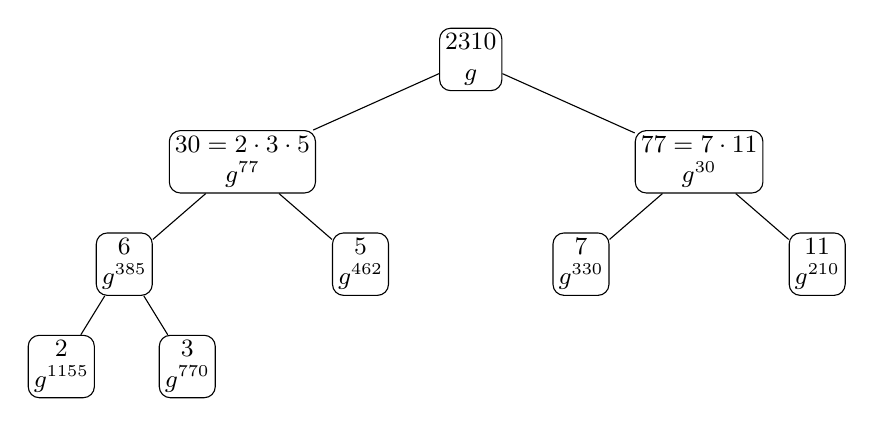
\begin{tikzpicture}[
    level distance=13mm,
    level 1/.style={sibling distance=58mm},
    level 2/.style={sibling distance=30mm},
    level 3/.style={sibling distance=16mm},
    every node/.style={draw, rounded corners, inner sep=2pt, font=\small, align=center}]
  \node {$2310$\\ $g$}
    child { node {$30 = 2 \cdot 3 \cdot 5$\\ $g^{77}$}
      child { node {$6$\\ $g^{385}$}
        child { node {$2$\\ $g^{1155}$} }
        child { node {$3$\\ $g^{770}$} } }
      child { node {$5$\\ $g^{462}$} } }
    child { node {$77 = 7 \cdot 11$\\ $g^{30}$}
      child { node {$7$\\ $g^{330}$} }
      child { node {$11$\\ $g^{210}$} } };
\end{tikzpicture}
\caption{Спуск по дереву произведений для $N = 2310 = 2 \cdot 3 \cdot 5 \cdot 7 \cdot 11$:
в узле с произведением $P_S$ находится $g^{N/P_S}$; например, $g^{77} \mapsto (g^{77})^{5} =
g^{385}$ и $(g^{77})^{6} = g^{462}$}
\label{l7:fig-tree}
\end{figure}

\begin{theorem}\label{l7:tree-correct}
Алгоритм~\ref{l7:alg-tree} возвращает $\ord g$ и выполняет
$\bigO\bigl(\log N \cdot (1 + \log \omega(N))\bigr) = \bigO(\log N \log\log N)$ групповых
операций.
\end{theorem}

\begin{proof}
\emph{Корректность.} Инвариант $h_S = g^{N/P_S}$ проверен выше индукцией по глубине узла;
в листьях $h_i = g^{N/Q_i}$. Цикл \textbf{пока} находит $k_i$ с $\ord h_i = q_i^{k_i}$
(порядок $h_i$ "--- степень $q_i$ по лемме~\ref{l7:prime-parts}, и $h_i^{q_i^k} = 1 \iff
q_i^{k_i} \mid q_i^k$). По лемме~\ref{l7:prime-parts} $\ord g = \prod_i q_i^{k_i}$.

\emph{Сложность спуска.} Во внутреннем узле $S$ выполняются два возведения в степени $P_R$ и
$P_L$, т.\,е. $\bigO(\log P_L + \log P_R + 1) = \bigO(\log P_S + 1)$ умножений. Узлы одного
уровня соответствуют непересекающимся множествам листьев, поэтому сумма $\log P_S$ по уровню не
превосходит $\log N$; уровней $\ceil{\log_2 r}$, всего узлов меньше $2r$. Итого
$\bigO(\log N \log r + r)$, и $r = \omega(N) \le \log_2 N$.

\emph{Сложность в листьях.} Не более $e_i$ возведений в степень $q_i$, т.\,е.
$\bigO(e_i \log q_i + e_i)$ умножений; в сумме $\bigO(\log N)$.

Наконец, $\omega(N) = \bigO(\log N / \log\log N)$, поэтому $\log \omega(N) = \bigO(\log\log N)$.
\end{proof}

Для сравнения: последовательное снижение "--- $\bigO(\Omega(N) \log N)$, раздельное
вычисление всех $h_i$ "--- $\bigO(\omega(N) \log N)$, дерево "--- $\bigO(\log N \log \omega(N))$
операций. Для криптографических $N$ (несколько тысяч бит) разница существенна, если у $N$ много
простых делителей; при $\omega(N) \le 2$ (например, $N = p - 1 = 2q$) все методы равноценны.

\taskexample{order-product-tree}

\checkyourself{Сколько возведений в степень выполнит алгоритм~\ref{l7:alg-reduction} для
$N = 2^{k}$ и элемента порядка $1$? порядка $N$? Как ведёт себя дерево произведений при
$r = 1$?}

\checkyourself{Что вернёт алгоритм~\ref{l7:alg-tree}, если $N$ не кратно $\ord g$? Можно
ли это обнаружить?}

\section{Цикличность группы \texorpdfstring{$\Znx{p}$}{(Z/pZ)*}}

\begin{lemma}\label{l7:roots}
Ненулевой многочлен $f$ степени $d$ с коэффициентами в поле $K$ имеет не более $d$ корней в $K$.
\end{lemma}

\begin{proof}
Индукция по $d$; при $d = 0$ корней нет. Если $f(a) = 0$, разделим с остатком:
$f(x) = (x - a) f_1(x) + c$, $c \in K$; подставляя $x = a$, получаем $c = 0$. Если $f(b) = 0$ и
$b \ne a$, то $(b - a) f_1(b) = 0$, и так как в поле нет делителей нуля, $f_1(b) = 0$. По
предположению индукции у $f_1$ ($\deg f_1 = d - 1$) не более $d - 1$ корней, у $f$ "--- не
более $d$.
\end{proof}

Условие «$K$ "--- поле» существенно: например, $x^2 - 1$ имеет в $\Zn{8}$ четыре корня
$1, 3, 5, 7$.

\begin{theorem}\label{l7:cyclic}
Любая конечная подгруппа $G$ мультипликативной группы поля циклическая. В частности, группа
$\Znx{p}$ ($p$ простое) и группа $\GF{q}^*$ любого конечного поля циклические.
\end{theorem}

\begin{proof}
Пусть $\abs{G} = n$ и $\psi(d)$ "--- число элементов порядка $d$ в $G$. По следствию
теоремы Лагранжа $\psi(d) = 0$ при $d \nmid n$, и $\sum_{d \mid n} \psi(d) = n$.

Покажем, что $\psi(d) \le \varphi(d)$. Если $\psi(d) = 0$, это верно. Пусть $a \in G$ имеет
порядок $d$. Все $d$ элементов $1, a, \dots, a^{d-1}$ подгруппы $\langle a \rangle$ различны и
являются корнями многочлена $x^d - 1$, у которого по лемме~\ref{l7:roots} не больше $d$ корней.
Значит, \emph{каждый} элемент порядка $d$ (он тоже корень $x^d - 1$) лежит в $\langle a \rangle$,
а в циклической группе $\langle a \rangle$ порядка $d$ элементов порядка $d$ ровно $\varphi(d)$
(следствие~\ref{l7:cyclic-count}). Итак, $\psi(d) \le \varphi(d)$.

Теперь по следствию~\ref{l7:cyclic-count}
\[
  n = \sum_{d \mid n} \psi(d) \le \sum_{d \mid n} \varphi(d) = n,
\]
поэтому все неравенства "--- равенства: $\psi(d) = \varphi(d)$ для каждого $d \mid n$. В
частности, $\psi(n) = \varphi(n) \ge 1$: в $G$ есть элемент порядка $n$, т.\,е. образующий.
\end{proof}

\begin{definition}
Целое $g$ называется \emph{первообразным корнем} по модулю $n$, если $\gcd(g, n) = 1$ и
$\ord g = \varphi(n)$ в $\Znx{n}$, т.\,е. класс $g$ порождает $\Znx{n}$.
\end{definition}

\begin{corollary}\label{l7:count-roots}
По простому модулю $p$ существуют первообразные корни, и их ровно $\varphi(p - 1)$ (среди
вычетов $1, \dots, p - 1$). Если $g$ "--- один из них, то все они "--- это $g^k \bmod p$ с
$1 \le k < p - 1$, $\gcd(k, p - 1) = 1$. Для каждого $d \mid p - 1$ сравнение
$x^d \equiv 1 \pmod p$ имеет ровно $d$ решений.
\end{corollary}

\begin{proof}
Первые два утверждения "--- теорема~\ref{l7:cyclic} и следствие~\ref{l7:cyclic-count}. Решения
$x^d = 1$ "--- элементы, порядок которых делит $d$; их $\sum_{d' \mid d} \varphi(d') = d$.
\end{proof}

Например, по модулю $11$ первообразный корень $2$, а $\varphi(10) = 4$ первообразных корня "---
$2^1, 2^3, 2^7, 2^9 \equiv 2, 8, 7, 6$.

\taskexample{primroot-all}

\checkyourself{Докажите, что произведение всех первообразных корней по простому модулю
$p > 3$ сравнимо с $1$. (Указание: $g^k$ и $g^{-k}$.)}

\section{Поиск первообразного корня}

\begin{theorem}[критерий первообразного корня]\label{l7:primroot-test}
Пусть $\gcd(g, n) = 1$, и $q_1, \dots, q_r$ "--- все простые делители $\varphi(n)$. Число $g$
является первообразным корнем по модулю $n$ тогда и только тогда, когда
\[
  g^{\varphi(n)/q_i} \not\equiv 1 \pmod n \qquad \text{для всех } i = 1, \dots, r.
\]
В частности, для простого $p$: $g$ "--- первообразный корень $\iff$ $g^{(p-1)/q} \not\equiv 1
\pmod p$ для всех простых $q \mid p - 1$.
\end{theorem}

\begin{proof}
По теореме Эйлера $g^{\varphi(n)} \equiv 1$, и утверждение есть лемма~\ref{l7:order-test} при
$m = \varphi(n)$.
\end{proof}

Проверка стоит $r = \omega(\varphi(n))$ возведений в степень, т.\,е.
$\bigO(\omega(\varphi(n)) \log n)$ умножений по модулю $n$ "--- \emph{при известном разложении}
$\varphi(n)$.

\begin{algorithm}[поиск наименьшего первообразного корня по модулю $p$]\label{l7:alg-primroot}
\begin{algorithmic}[1]
\Require простое $p > 2$ и разложение $p - 1 = \prod_{i=1}^r q_i^{e_i}$.
\Ensure наименьший первообразный корень $g$.
\For{$g = 2, 3, \dots$}
  \If{$g$ "--- полный квадрат} \State \textbf{перейти} к следующему $g$ \Comment{не корень}
  \EndIf
  \If{$g^{(p-1)/q_i} \not\equiv 1 \pmod p$ для всех $i$} \State \Return $g$ \EndIf
\EndFor
\end{algorithmic}
\end{algorithm}

Квадраты пропускаются, так как при $g = h^2$ имеем $g^{(p-1)/2} = h^{p-1} \equiv 1$. По тем же
соображениям, если $g$ не первообразный корень, то не являются ими и его степени, но на практике
эту экономию обычно не используют. Для составного $n$ (если корни существуют, см. следующий
раздел) алгоритм тот же: $p - 1$ заменяется на $\varphi(n)$, а числа $g$ с $\gcd(g, n) > 1$
пропускаются.

\begin{example}\label{l7:ex-41}
$p = 41$, $p - 1 = 40 = 2^3 \cdot 5$, проверяемые показатели $40/2 = 20$ и $40/5 = 8$:
\[
\begin{array}{c|cc|l}
  g & g^{20} & g^{8} & \\ \hline
  2 & 1 & & \text{нет} \\
  3 & 40 & 1 & \text{нет} \\
  4 & & & = 2^2 \\
  5 & 1 & & \text{нет} \\
  6 & 40 & 10 & \text{первообразный корень}
\end{array}
\]
Наименьший первообразный корень по модулю $41$ "--- число $6$; всего их $\varphi(40) = 16$.
\end{example}

\taskexample{primroot-search}

\paragraph{Стоимость поиска.} Доля первообразных корней среди вычетов равна
$\varphi(p - 1)/(p - 1) = \prod_{q \mid p - 1}(1 - 1/q)$. Известно
(\cite[теорема~328]{hardy-wright}, без доказательства), что
$\varphi(m)/m \ge c/\ln\ln m$ для некоторой константы $c > 0$ и всех $m \ge 3$. Если считать
кандидатов $g = 2, 3, \dots$ «случайными» (это эвристика, а не теорема), то в среднем
понадобится $(p - 1)/\varphi(p - 1) = \bigO(\log\log p)$ кандидатов, т.\,е.
\[
  \bigO\bigl(\log\log p \cdot \omega(p - 1) \cdot \log p\bigr)
\]
умножений по модулю $p$. Опыт подтверждает, что наименьший первообразный корень очень мал:
например, для всех $p < 10^4$ он не превосходит $31$, а число $2$ является первообразным
корнем примерно для $37{,}4\,\%$ простых (гипотеза Артина: доля равна константе Артина
$0{,}3739\ldots$; доказано Хули при условии обобщённой гипотезы Римана). Строгие оценки
слабее: $g(p) = \bigO(p^{1/4 + \varepsilon})$ (Бёрджесс) и, при обобщённой гипотезе Римана,
$g(p) = \bigO(\log^6 p)$ (Шуп) "--- без доказательства.

Главная трудность "--- не перебор, а \emph{разложение $p - 1$}: без него неизвестно, как
проверить, что $g$ "--- образующий. Поэтому в криптографии простое $p$ выбирают вместе с
разложением $p - 1$, чаще всего \emph{безопасное простое} $p = 2q + 1$ ($q$ простое).

\begin{proposition}\label{l7:safe-prime}
Пусть $p = 2q + 1$, $p$ и $q$ "--- простые нечётные, $2 \le g \le p - 2$. Тогда $g$ "---
первообразный корень по модулю $p \iff g^q \equiv -1 \pmod p$; в противном случае
$g^q \equiv 1$ и $\ord g = q$.
\end{proposition}

\begin{proof}
Простые делители $p - 1$ "--- это $2$ и $q$. Условие $g^{(p-1)/q} = g^2 \ne 1$ выполнено, так
как $x^2 = 1$ имеет в поле только корни $\pm 1$. Значит, по теореме~\ref{l7:primroot-test}
$g$ "--- первообразный корень $\iff g^q \ne 1$. Так как $(g^q)^2 = 1$, то $g^q = \pm 1$. Если
$g^q = 1$, то $\ord g \mid q$ и $\ord g \ne 1$, т.\,е. $\ord g = q$.
\end{proof}

Например, $p = 23 = 2 \cdot 11 + 1$: $2^{11} \equiv 3^{11} \equiv 1$, $4 = 2^2$, $5^{11}
\equiv 22 \equiv -1 \pmod{23}$, поэтому наименьший первообразный корень по модулю $23$ "---
$5$, а $2$ и $3$ имеют порядок $11$.

\checkyourself{Почему для безопасного простого $p = 2q + 1$ ровно половина (с точностью до
одного элемента) вычетов $2, \dots, p - 2$ "--- первообразные корни?}

\checkyourself{Пусть $g$ "--- не первообразный корень по модулю $p$. Может ли $g^3$ оказаться
первообразным корнем? А $g^{-1}$?}

\section{Первообразные корни по составному модулю}

Какие группы $\Znx{n}$ циклические? Ответ дал Гаусс.

\begin{theorem}[Гаусс]\label{l7:gauss}
Первообразные корни по модулю $n \ge 1$ существуют тогда и только тогда, когда
\[
  n \in \{1, 2, 4, p^k, 2p^k\}, \qquad p \text{ "--- нечётное простое}, \ k \ge 1.
\]
Если они существуют, их ровно $\varphi(\varphi(n))$.
\end{theorem}

Число корней следует из следствия~\ref{l7:cyclic-count}. Для $n = 1, 2, 4$ первообразные корни
"--- это $1$ (группа $\Znx{2}$ и группа из одного элемента), $1$ и $3$ ($\Znx{4} = \{1, 3\}$,
$\ord 3 = 2$). Остальное докажем в несколько шагов.

\subsection{Модули \texorpdfstring{$p^k$}{p\^{}k}}

\begin{lemma}\label{l7:lift-step}
Пусть $p$ нечётное простое, $k \ge 1$ и $x = 1 + t p^k$, $p \nmid t$. Тогда
$x^p = 1 + t' p^{k+1}$, где $t' \equiv t \pmod p$; в частности, $p \nmid t'$.
\end{lemma}

\begin{proof}
По биному Ньютона
\[
  x^p = 1 + p \cdot t p^k + \binom p2 t^2 p^{2k} + \sum_{j \ge 3} \binom pj t^j p^{jk}.
\]
Второе слагаемое равно $t p^{k+1}$. Так как $p$ нечётно, $p \mid \binom p2 = p(p-1)/2$, и третье
слагаемое делится на $p^{2k+1}$, а остальные "--- на $p^{3k}$; оба показателя не меньше $k + 2$
при $k \ge 1$. Поэтому $x^p \equiv 1 + t p^{k+1} \pmod{p^{k+2}}$.
\end{proof}

\begin{theorem}\label{l7:pk}
Пусть $p$ нечётное простое, $g$ "--- первообразный корень по модулю $p$.
\begin{enumerate}
  \item Хотя бы одно из чисел $g$, $g + p$ удовлетворяет условию
    $g^{p-1} \not\equiv 1 \pmod{p^2}$.
  \item Если $g^{p-1} \not\equiv 1 \pmod{p^2}$, то $g$ "--- первообразный корень по модулю
    $p^k$ для всех $k \ge 1$.
\end{enumerate}
Обратно, первообразный корень по модулю $p^k$, $k \ge 2$, является первообразным корнем по
модулю $p$ и удовлетворяет $g^{p-1} \not\equiv 1 \pmod{p^2}$.
\end{theorem}

\begin{proof}
1. Пусть $g^{p-1} \equiv 1 \pmod{p^2}$. По биному
\[
  (g + p)^{p-1} \equiv g^{p-1} + (p - 1) g^{p-2} p \equiv 1 - p g^{p-2} \pmod{p^2},
\]
и $p g^{p-2} \not\equiv 0 \pmod{p^2}$, так как $p \nmid g$. Значит, $(g + p)^{p-1}
\not\equiv 1 \pmod{p^2}$; при этом $g + p \equiv g \pmod p$ "--- тоже первообразный корень
по модулю $p$.

2. Пусть $g^{p-1} = 1 + tp$, $p \nmid t$. Применяя лемму~\ref{l7:lift-step} $j$ раз, получаем
$g^{p^j(p-1)} = 1 + t_j p^{j+1}$, $p \nmid t_j$. Пусть $d = \ord g$ по модулю $p^k$; тогда
$d \mid \varphi(p^k) = p^{k-1}(p - 1)$. Из $g^d \equiv 1 \pmod{p^k}$ следует
$g^d \equiv 1 \pmod p$, т.\,е. $(p - 1) \mid d$ (так как $g$ "--- первообразный корень по
модулю $p$). Значит, $d = p^j (p - 1)$ для некоторого $j \le k - 1$. Если бы $j \le k - 2$, то
$g^{p^{k-2}(p-1)} \equiv 1 \pmod{p^k}$, а это противоречит равенству
$g^{p^{k-2}(p-1)} = 1 + t_{k-2} p^{k-1}$, $p \nmid t_{k-2}$. Итак, $d = \varphi(p^k)$.

Обратное утверждение. Приведение по модулю $p^j$ ($j \le k$) "--- сюръективный гомоморфизм
$\Znx{p^k} \to \Znx{p^j}$, и образ образующего порождает весь $\Znx{p^j}$. Значит, $g$ "---
первообразный корень по модулям $p$ и $p^2$, а тогда $\ord_{p^2} g = p(p - 1)$ и
$g^{p-1} \not\equiv 1 \pmod{p^2}$.
\end{proof}

Итак, $g$ "--- первообразный корень по модулю $p^k$ ($k \ge 2$) тогда и только тогда, когда
$g$ "--- первообразный корень по модулю $p$ и $g^{p-1} \not\equiv 1 \pmod{p^2}$. Например,
$3$ "--- первообразный корень по модулю $7$, и $3^6 = 729 \equiv 43 \not\equiv 1 \pmod{49}$,
поэтому $3$ "--- первообразный корень по модулям $7^k$ для всех $k$. Исключительный случай
$g^{p-1} \equiv 1 \pmod{p^2}$ редок, но встречается: $5$ "--- наименьший первообразный корень
по модулю $p = 40487$, но $5^{40486} \equiv 1 \pmod{40487^2}$, так что по модулю $40487^2$
нужно брать, например, $5 + 40487 = 40492$.

\subsection{Модули \texorpdfstring{$2p^k$}{2p\^{}k}}

\begin{proposition}\label{l7:2pk}
Пусть $g$ "--- первообразный корень по модулю $p^k$ ($p$ нечётное простое). Тогда из чисел
$g$, $g + p^k$ нечётное является первообразным корнем по модулю $2p^k$.
\end{proposition}

\begin{proof}
Пусть $g'$ "--- нечётное из этих чисел; $g' \equiv g \pmod{p^k}$ и $\gcd(g', 2p^k) = 1$. По
китайской теореме об остатках $x \equiv 1 \pmod{2p^k} \iff x \equiv 1 \pmod 2$ и
$x \equiv 1 \pmod{p^k}$. Для нечётного $x$ первое выполнено всегда, поэтому порядок $g'$ по
модулю $2p^k$ совпадает с порядком по модулю $p^k$, т.\,е. равен
$\varphi(p^k) = \varphi(2p^k)$.
\end{proof}

Например, $2$ "--- первообразный корень по модулю $9$, но чётно; $2 + 9 = 11$ "---
первообразный корень по модулю $18$. (Наименьший первообразный корень по модулю $18$ "---
число $5$.)

\subsection{Остальные модули: корней нет}

\begin{lemma}\label{l7:no-roots}
\begin{enumerate}
  \item Если $n = ab$, $\gcd(a, b) = 1$, $a > 2$, $b > 2$, то $x^{\varphi(n)/2} \equiv 1
    \pmod n$ для всех $x$, взаимно простых с $n$.
  \item Если $n = 2^k$, $k \ge 3$, то $x^{2^{k-2}} \equiv 1 \pmod{2^k}$ для всех нечётных $x$.
\end{enumerate}
В обоих случаях порядок любого элемента $\Znx{n}$ не больше $\varphi(n)/2$, и первообразных
корней нет.
\end{lemma}

\begin{proof}
1. При $m > 2$ число $\varphi(m)$ чётно: если у $m$ есть нечётный простой делитель $q$, то
$(q - 1) \mid \varphi(m)$, иначе $m = 2^j$, $j \ge 2$, и $\varphi(m) = 2^{j-1}$. Так как
$\varphi(n) = \varphi(a)\varphi(b)$,
\[
  x^{\varphi(n)/2} = \bigl(x^{\varphi(a)}\bigr)^{\varphi(b)/2} \equiv 1 \pmod a, \qquad
  x^{\varphi(n)/2} = \bigl(x^{\varphi(b)}\bigr)^{\varphi(a)/2} \equiv 1 \pmod b,
\]
и по китайской теореме об остатках $x^{\varphi(n)/2} \equiv 1 \pmod{ab}$.

2. Индукция по $k$. При $k = 3$: $x^2 - 1 = (x - 1)(x + 1)$ "--- произведение двух соседних
чётных чисел, одно из которых делится на $4$, поэтому $8 \mid x^2 - 1$. Если
$x^{2^{k-2}} = 1 + t 2^k$, то $x^{2^{k-1}} = 1 + t 2^{k+1} + t^2 2^{2k} \equiv 1
\pmod{2^{k+1}}$.
\end{proof}

\begin{proof}[Доказательство теоремы~\ref{l7:gauss}]
Существование для $1, 2, 4$ проверено выше, для $p^k$ "--- теорема~\ref{l7:pk} (вместе с
теоремой~\ref{l7:cyclic} для $k = 1$), для $2p^k$ "--- утверждение~\ref{l7:2pk}.

Пусть $n$ не входит в список. Если у $n$ нет нечётных простых делителей, то $n = 2^k$, $k \ge 3$,
и применим пункт~2 леммы~\ref{l7:no-roots}. Иначе пусть $p$ "--- нечётный простой делитель,
$b = p^{v_p(n)}$, $a = n/b$. Тогда $\gcd(a, b) = 1$, $b \ge 3$, а $a \ne 1$ (иначе
$n = p^k$) и $a \ne 2$ (иначе $n = 2p^k$), т.\,е. $a > 2$; применим пункт~1.
\end{proof}

Например, по модулю $8$ все нечётные $x$ удовлетворяют $x^2 \equiv 1$, а в $\Znx{15}$
(порядок $8$) максимальный порядок элемента равен $4$.

\taskexample{primroot-none}

\subsection{Функция Кармайкла}

\begin{definition}
\emph{Функция Кармайкла} $\lambda(n)$ "--- наименьшее $L \ge 1$, для которого $x^L \equiv 1
\pmod n$ при всех $x$, взаимно простых с $n$ (\emph{показатель} группы $\Znx{n}$).
\end{definition}

\begin{theorem}\label{l7:carmichael}
$\lambda(2) = 1$, $\lambda(4) = 2$, $\lambda(2^k) = 2^{k-2}$ при $k \ge 3$,
$\lambda(p^k) = \varphi(p^k) = p^{k-1}(p - 1)$ для нечётного простого $p$, и
\[
  \lambda\bigl(p_1^{k_1} \cdots p_s^{k_s}\bigr) = \lcm\bigl(\lambda(p_1^{k_1}), \dots,
  \lambda(p_s^{k_s})\bigr).
\]
Кроме того, в $\Znx{n}$ есть элемент порядка $\lambda(n)$. В частности, первообразный корень по
модулю $n$ существует $\iff \lambda(n) = \varphi(n)$.
\end{theorem}

\begin{proof}
Для $p^k$ с нечётным $p$, а также для $2$ и $4$ группа циклическая, поэтому $\lambda$ равна
порядку образующего $\varphi(p^k)$. Для $2^k$, $k \ge 3$, по лемме~\ref{l7:no-roots}
$\lambda(2^k) \mid 2^{k-2}$. С другой стороны, если $x = 1 + t 2^m$, $m \ge 2$, $t$ нечётно,
то $x^2 = 1 + t 2^{m+1} + t^2 2^{2m} \equiv 1 + t 2^{m+1} \pmod{2^{m+2}}$ (так как
$2m \ge m + 2$). Начиная с $5 = 1 + 2^2$, получаем $5^{2^j} = 1 + t_j 2^{j+2}$ с нечётным $t_j$. Значит, $5^{2^{k-3}} \not\equiv 1 \pmod{2^k}$
и $\ord 5 = 2^{k-2}$.

Общий случай. По китайской теореме об остатках $x^L \equiv 1 \pmod n$ тогда и только тогда,
когда $x^L \equiv 1 \pmod{p_i^{k_i}}$ для всех $i$, т.\,е. (так как $\lambda(p_i^{k_i})$ "---
порядок некоторого элемента, а все порядки его делят) когда $\lambda(p_i^{k_i}) \mid L$ для
всех $i$. Наименьшее такое $L$ "--- это $\lcm$. Элемент порядка $\lambda(n)$: выберем $x_i$ порядка
$\lambda(p_i^{k_i})$ по модулю $p_i^{k_i}$ и склеим их по китайской теореме; порядок $x$ по
модулю $n$ равен $\lcm$ порядков $x_i$, т.\,е. $\lambda(n)$.
\end{proof}

Например, $\lambda(15) = \lcm(2, 4) = 4 < \varphi(15) = 8$, $\lambda(24) = \lcm(2, 2) = 2$:
все $\varphi(24) = 8$ элементов $\Znx{24}$ удовлетворяют $x^2 = 1$. Функция Кармайкла появится
ещё в лекции~8 (числа Кармайкла $n$, для которых $\lambda(n) \mid n - 1$, обманывают тест
Ферма) и в лекции~9 (максимальный период мультипликативного конгруэнтного генератора по
модулю $m$ равен $\lambda(m)$).

\checkyourself{Найдите $\lambda(100)$ и $\varphi(100)$. Почему $\lambda(n)$ всегда делит
$\varphi(n)$?}

\section{Образующие для протокола Диффи"--~Хеллмана}

Подведём итог для выбора параметров протокола Диффи"--~Хеллмана в $\Znx{p}$.
\begin{enumerate}
  \item Порядок $\ord g$ должен иметь большой простой делитель (алгоритм Полига"--~Хеллмана,
    второй семестр), поэтому $p$ генерируют вместе с разложением $p - 1$; стандартный выбор "---
    безопасное простое $p = 2q + 1$.
  \item Первообразный корень $g$ (порядок $2q$) проверяется одним возведением в степень
    (утверждение~\ref{l7:safe-prime}). Однако он «выдаёт» чётность секретного показателя:
    $A^q = (g^q)^a = (-1)^a$, т.\,е. Ева по $A = g^a$ узнаёт $a \bmod 2$.
  \item Поэтому чаще работают в подгруппе \emph{квадратов} порядка $q$: $g = h^2 \bmod p$ при
    $h \ne \pm 1$ имеет порядок ровно $q$ (утверждение~\ref{l7:safe-prime}: $g^q = h^{2q} = 1$,
    $g \ne 1$). Порядок подгруппы простой, и малых множителей, через которые утекала бы
    информация о показателе, нет. Например, в группах RFC~3526 (протокол IKE) $g = 2$ и $p$
    "--- безопасное простое с $p \equiv 7 \pmod 8$; при таком $p$ число $2$ является квадратом
    (это следует из закона взаимности для символа Лежандра, второй семестр) и порождает
    подгруппу порядка $q$.
  \item Получив от партнёра $B$, полезно проверить $B \ne \pm 1$ и $B^q = 1$ (элемент лежит в
    нужной подгруппе) "--- это снова проверка порядка по лемме~\ref{l7:order-test}.
\end{enumerate}

\checkyourself{Пусть $p = 2q + 1$ и $g$ "--- первообразный корень. Сколько элементов порядка $q$
в $\Znx{p}$? Как выразить их все через $g$?}

\checkyourselfsection

\begin{furtherreading}
  \readitem[разд.~2.15]{galbraith}{вычисление порядка элемента (в том числе с деревом
    произведений), поиск образующих}
  \readitem[разд.~1.4, 2.2--2.3]{hps}{первообразные корни, порядок элемента и протокол
    Диффи"--~Хеллмана}
  \readitem[гл.~4]{ireland-rosen}{строение группы $\Znx{n}$, первообразные корни по
    модулям $p^k$, $2p^k$; отсутствие корней по остальным модулям}
  \readitem[гл.~VI]{vinogradov}{первообразные корни и индексы}
  \readitem[гл.~11]{shoup}{поиск образующего группы $\Znx{p}$ и вероятностный анализ}
  \readitem[разд.~3.2.1.2]{knuth-taocp2}{функция Кармайкла $\lambda(n)$ и период
    конгруэнтного генератора}
  \readitem{cp-algorithms}{статья «Primitive Root»: алгоритм поиска и реализация}
  \readitem{msu-ent}{курс элементарной теории чисел МГУ: порядок по модулю, первообразные корни}
\end{furtherreading}
\end{lecture}
